
\documentclass[11pt,titlepage]{article}
%%%%%%%%%%%%%%%%%%%%%%%%%%%%%%%%%%%%%%%%%%%%%%%%%%%%%%%%%%%%%%%%%%%%%%%%%%%%%%%%%%%%%%%%%%%%%%%%%%%%%%%%%%%%%%%%%%%%%%%%%%%%

\usepackage{epsfig}
\usepackage{times}

\textwidth=6.5in \textheight=9.25in
 \topmargin=-0.5in
\evensidemargin=0in \oddsidemargin=0in
\baselineskip=12pt \parskip=8pt

\begin{document}
\bibliographystyle{prsty} % Choose Phys. Rev. stylle for bibliography
\title{\textsf{High Threshold Cerenkov Counter}}
\author{Valery Kubarovsky\\
{\it \small Rensselaer Polytechnic Institute/Jlab}\\
Ivan Bedlinsky\\
{\it \small Institute of Theoretical and Experimental Physics, Moscow}\\
Pavel Degtyarenko\\
{\it \small Jlab}\\
Alexsandr Glamazdin\\
{\it \small Kharkov Institute of Physics and Technology, Kharkov}}
\date{\today }
\maketitle
\clearpage

\section{Introduction}

\noindent{\bf High Threshold CLAS12 \v Cerenkov Detector.} The RPI group has been  fully 
committed to the JLab upgrade during  all its phases. At this time our primary hardware 
responsibility is the high threshold threshold \v Cerenkov detector (HTCC) which will 
be an integral component of the CLAS12 spectrometer. A rendering of the CLAS12 \v Cerenkov  
in the context of the overall detector, and its optical design  is shown in Fig.~\ref{clas12_mirror}
left panel.
Right panel shows the mirror prototype.

16 photomultiplier tubes (PMT) will be used to collect the \v Cerenkov light from one sector.
So  16x6=96 PMT's will be used in total.
Each PMT will be  surrounded by a high magnetic permeability shielding (mu-metal). 
We consider two types of the 5'' photomultiplier: Burle 8854 or Photonic 4500.
This is a 129 mm (5 inch) diameter, 
having a bi-alkali photocathode of high quantum 
efficiency and an extremely high gain cesiated gallium phosphide first dynode followed 
by high stability copper beryllium dynodes in the succeeding stages. 
The high gain first dynode permits the direct observation of peaks corresponding to one 
photoelectron.

%-------------------------------------------
 \begin{figure}
\hspace{0.5cm}
 \begin{centering}
  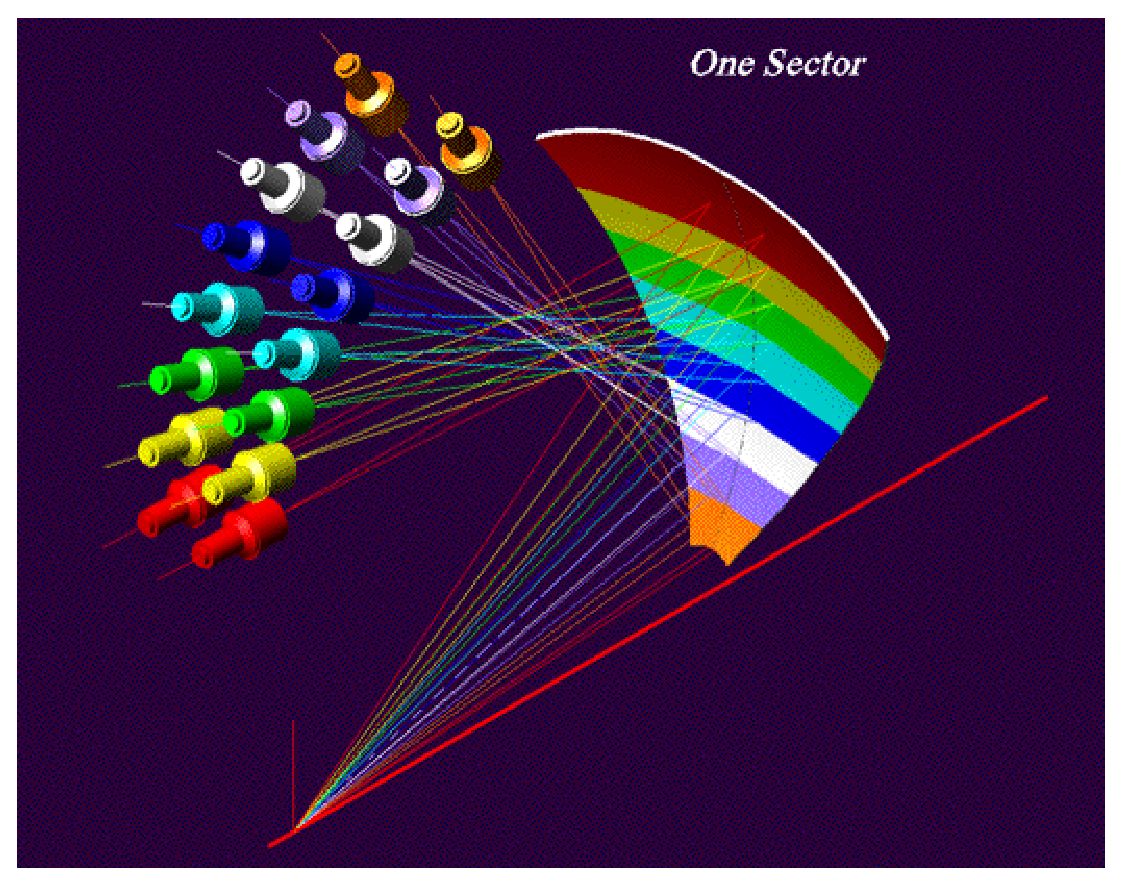
\includegraphics[height=5.5cm]{CLAS12-optics.eps}
 \includegraphics[height=5.5cm]{cerenk-mirror.epsi}
 \hspace{0.1cm}

 \caption{\label{clas12_mirror}
Left panel: Current optical design for the HTCC. Right panel: the mirror prototype.
 }
 \end{centering}
 \end{figure}

There are two types of PMT under investigation: with UV-glass input window
and with quartz input window.

The UV-glass window features high quantum efficiency (22.5\% at 385 nm) and 
ultraviolet response up to $\lambda\sim$220 nm. The number of photons from the 
\v Cerenkov light is proportional to $1/\lambda^2$, so it's important to have 
a extended response in UV light. The quartz window is transparent up to the 
$\lambda\sim$180 nm. So it is more efficient for the detection of the \v Cerenkov light.
However the PMT with quartz window is much more expensive.

We designed the experimental set up to measure 
the ratio of the average number of photoelectrons
collected by these two types PMT's illuminated by the \v Cerenkov light. We are using two methods to
measure this ratio.

\section{Cosmic Ray Stand}

\noindent

We constructed Cosmic Ray Stand (CRS) which has the source of the \v Cerenkov light.
The final goal is to compare the response of PMT with UV-glass and quartz input window 
to \v Cerenkov light.
The test detector (Fig.~\ref{clas12_scheme}) consists of alternate layers of scintillator and quartz plates
(150x150x5 mm). The \v Cerenkov 
light is produced in the quartz plates
when irradiated with cosmic muons. The light is directed to the photomultiplier
tubes which are being tested, and their responses electronically analyzed. During the 
data taking we are accumulating data for all tubes and make our selection
based on the results. 
Two 5x5 cm$^2$ trigger counters produce trigger signal that goes to the data acquisition system.
The signal from all 6 PMTs: trigger counters, scintillator counters and 
\v Cerenkov counters go to Amplitude to Digital Converters (ADC) for further analysis.
Fig.~\ref{stand_raw} presented the ADC distributions. 

%-------------------------------------------
 \begin{figure}
 \vspace{1.cm}
 \begin{centering}
  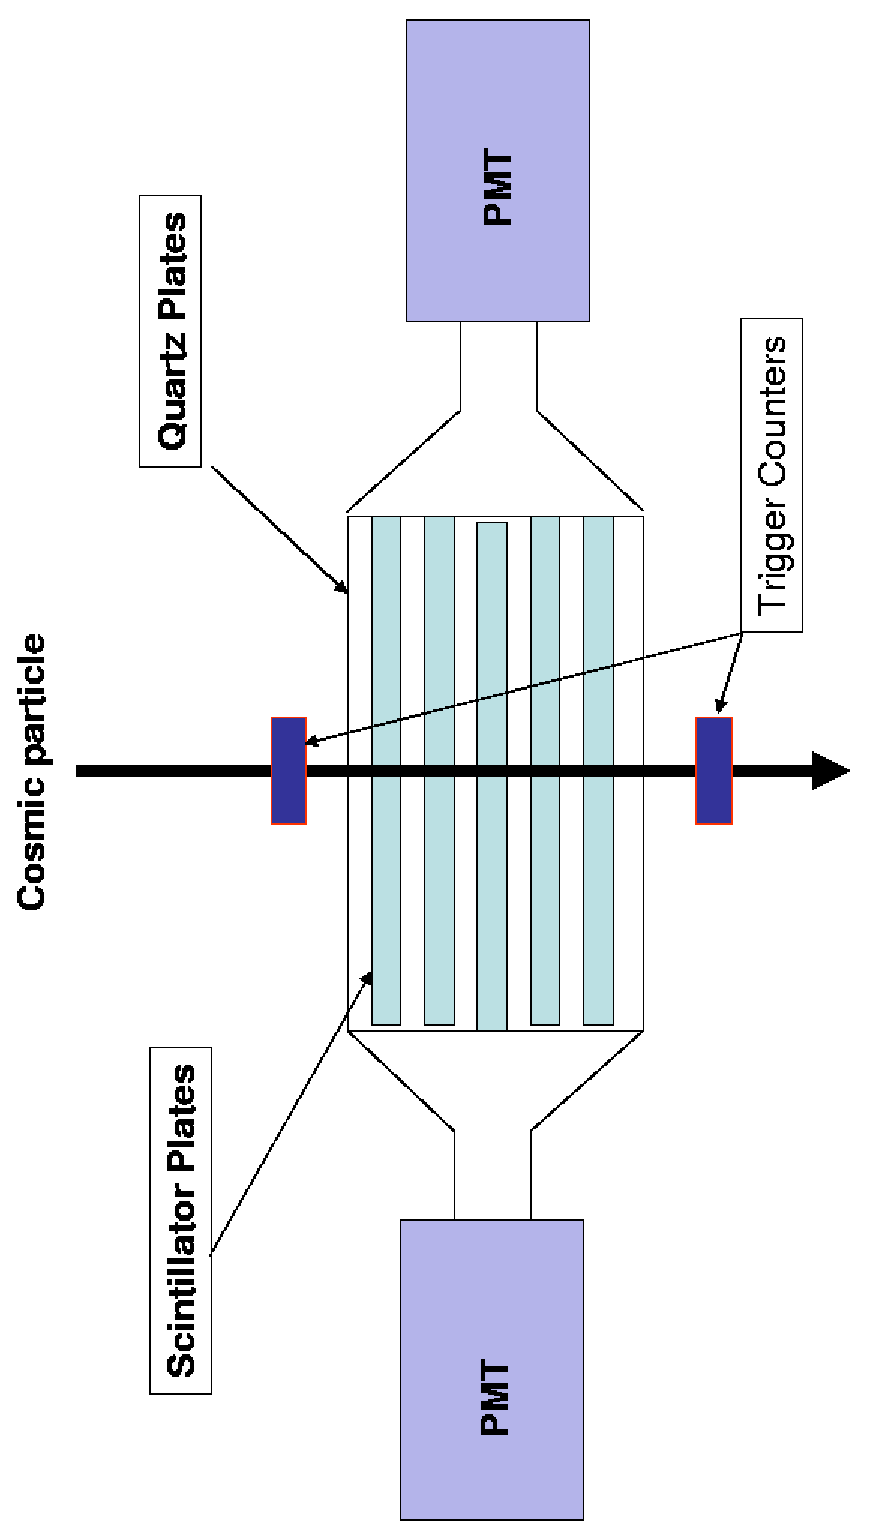
\includegraphics[height=7.0cm,angle=-90]{sc.eps}
 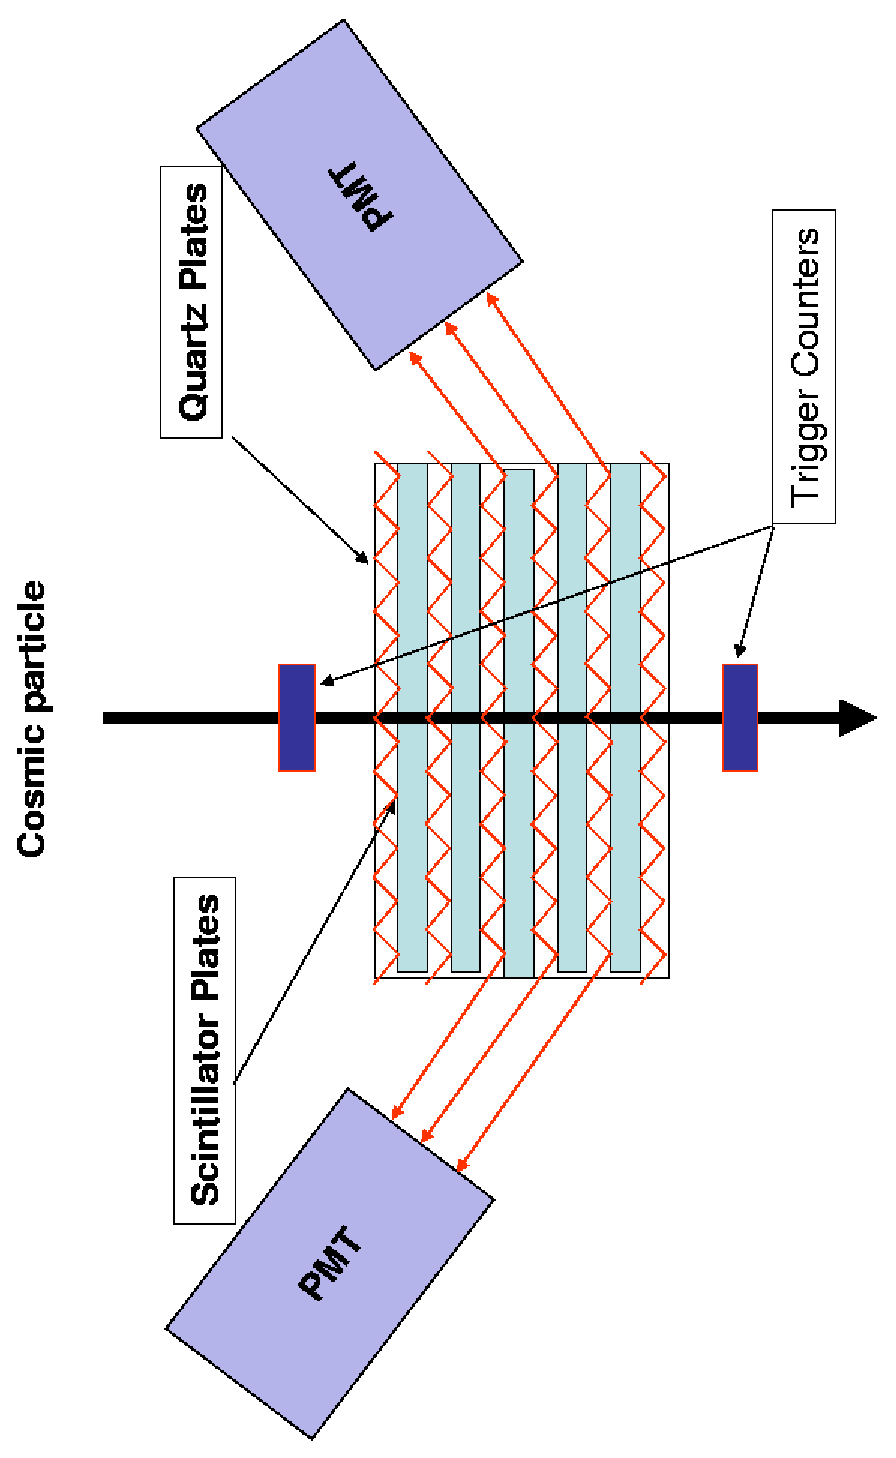
\includegraphics[height=7.0cm,angle=-90]{cc.eps}
 \hspace{0.1cm}
 \caption{\label{clas12_scheme}
Left panel: view of the cosmic ray stand from the side of the \v Cerenkov counters.
Right panel: view of the cosmic ray stand from the side of the scintillation counters.
 }
 \end{centering}
 \end{figure}

%-------------------------------------------
 \begin{figure}
 \vspace{0.5cm}
 \begin{centering}
 \includegraphics[height=5.5cm]{cerenk-test.epsi}
 \includegraphics[height=5.5cm]{cerenk-daq.epsi}
 \vspace{0.5cm}
 \caption{\label{clas12_stand_daq}
Left panel: photo of the cosmic ray stand.
Right panel: photo of the data acquisition of the cosmic ray stand.
 }
 \end{centering}
 \end{figure}


The detector has three main subsystems.
\begin{itemize}
\item Trigger Counters MM1 and MM2. These counters are used to produce the trigger signal
when cosmic muons cross the detector. The size of the trigger counters is small enough
in comparison with the size of the scintillator and quartz plates to reduce the
fluctuation of the produced \v Cerenkov photons.
\item Scintillator Counters SC1 and SC2 collect light from the scintillator plates.
These counters serve as an additional prove that cosmic muon cross the sandwich
of the detector. We cut out the events with bad ADC signal in the scintillator counters.
\item \v Cerenkov Counters CC1 and CC2. These counter collect the light from quartz plates. One of the
counters (CC2) serve as reference device. The CC1 place is used to study the  PMT's.
\end{itemize}



%-------------------------------------------

 \begin{figure}
 \hspace{0.5cm}
 \begin{centering}
  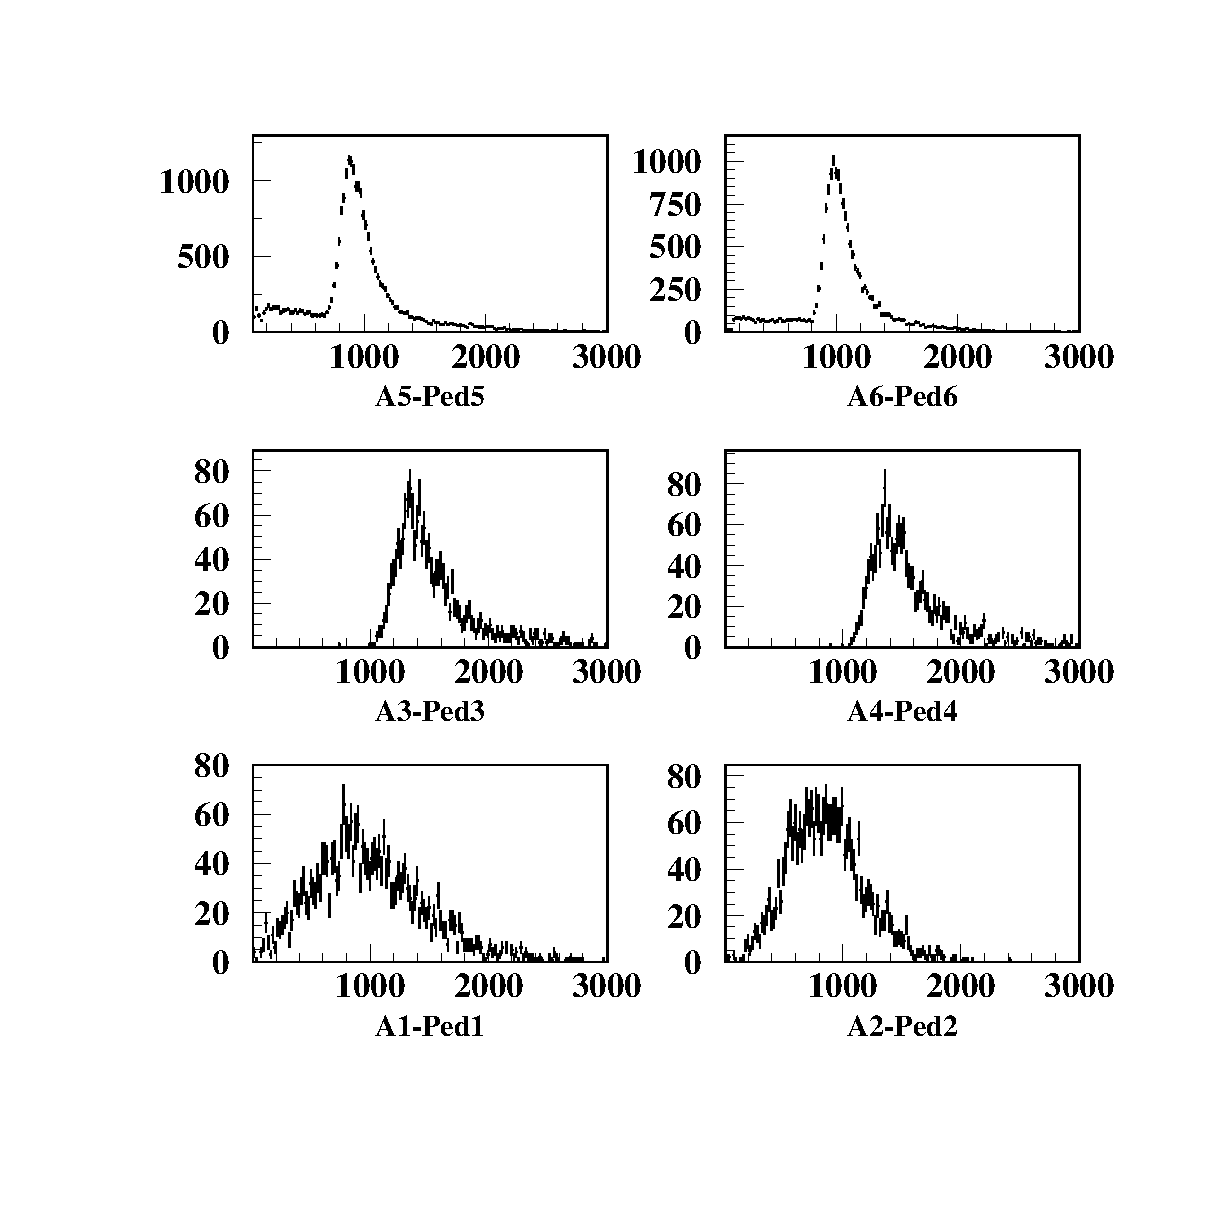
\includegraphics[height=12.5cm]{raw_adc.eps}
 \vspace{-1.0cm}
 \caption{\label{stand_raw}
The ADC spectra for the trigger counters, scintillator counters and \v Cerenkov counters.
}
 \end{centering}
 \end{figure}

The upper panels of Fig. \ref{stand_raw} show the ADC distributions for the trigger counters for the events
with amplitude in the scintillator counters (middle panels) more than 1000 counts.
Clear signals form the cosmic muons are seen in  both trigger counters. The events with 
lower amplitudes correspond to the case when the particle crosses the light guide.

The middle panels show the ADC distributions for the scintillator counters for the events
with amplitude in the trigger counters (top  panels) more than 800 counts.
Clear signals form the cosmic particles are seen in  both counters with good photostistics.

The bottom panels show the ADC distributions for the \v Cerenkov counters for the events
with amplitude in the trigger counters (top  panels) more than 800 counts.
Clear signals form the cosmic muons are seen in both counters.

The even selection criteria are:

  {$$ADC(MM1)> 800, ADC(MM2)> 800$$}
  {$$ADC(SC1)> 1000, ADC(SC2)> 1000$$} 


\section{Calibration of the ADC scale}

We need to calibrate the ADC spectrum  in the terms of photoelecrons for the PMT comparison.
We used two independent methods for this task.

The first calibration method uses the position of one-photoelectron peak from the real data.
Fig.~\ref{one_photon} presents the ADC distributions of the \v Cerenkov counter in the
region near pedestal. We eliminate the PMT with light emission diode (LED) with low intensity.
The peak near the pedestal corresponds to one-photoelectron signal.

The second method uses light emission diodes signal  to calibrate the scale.
PMT was eliminated with the light of LED with variable intensity.
The ADC spectra was fitted using Poisson function with two parameters.

$$ N=Cons{\mu^xe^{-x}\over\Gamma[x+1]}$$

where $Cons$ is the number of counts per channel, x is the SDC channel, 
and $\Gamma$ is the gamma function, given by

$$\Gamma(x)=\int^\infty_0t^{x-1}e^{-t}dt$$
 
The fit gives the calibration scale (the one-photoelectron position in terms of ADC counts) and
the average number of the photoelectrons in the distributions.
Fig.~\ref{uv_1_fit},\ref{uv_2_fit},\ref{qt_1_fit} present the ADC spectra for different amount of LED light
for 3 different PMT's. 

Fig~\ref{uv_1_result},\ref{uv_2_result},\ref{qt_1_result}  present the dependence of the average ADC value
as a function of the fitted number of photoelectrons for three different PMT
as a function of the ADC value.
The linear dependence shows that this method is self-concerted in all three PMTs.

These two methods give very close results.

The normalized spectrum is shown in Fig.~\ref{stand_phe}.
This is the final distributions that will be used for the PMT selection.
The PMT with better quantum efficiency to the \v Cerenkov radiation
picks up more photoelecrons.

%-------------------------------------------

 \begin{figure}
 \hspace{0.5cm}
 \begin{centering}
  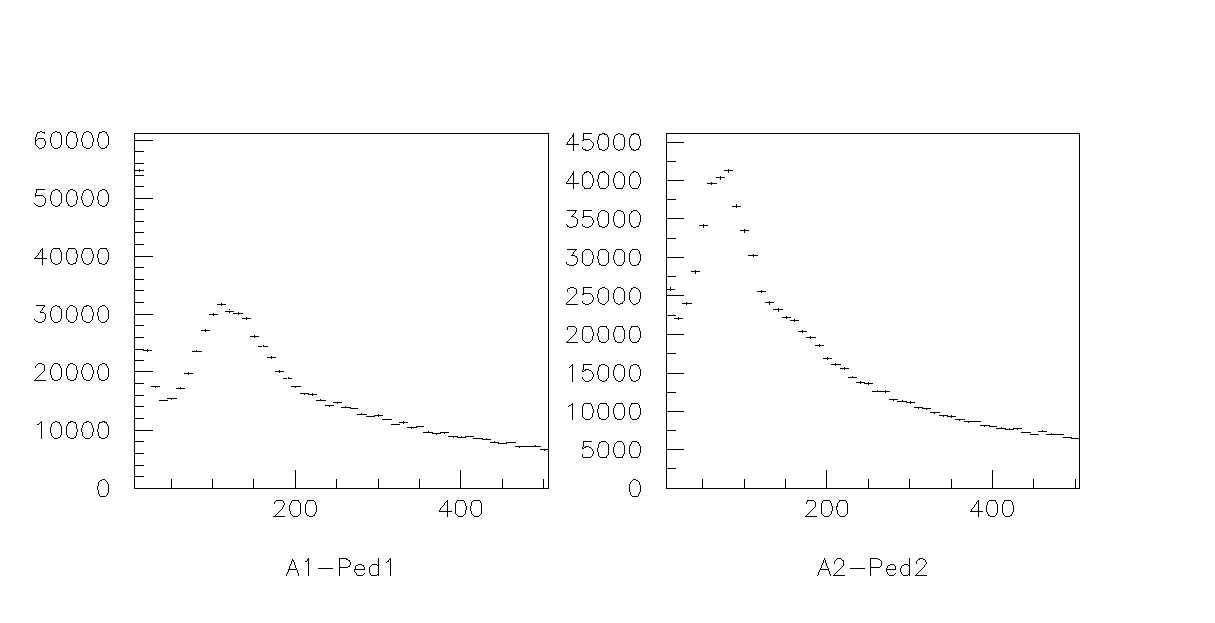
\includegraphics[height=7.5cm]{one_photon.eps}
 \vspace{0.5cm}
 \caption{\label{one_photon}
The ADC spectra of the \v Cerenkov counter. One-photoelectron peak is clearly seen. }
\end{centering}
 \end{figure}

%-------------------------------------------

% \begin{figure}
% \hspace{0.5cm}
% \begin{centering}
%  \includegraphics[height=12.5cm]{k02471_led.eps}
% \vspace{0.5cm}
% \caption{\label{led_spectra}
%The LED spectra of the \v Cerenkov counter. The spectra were fit by Poisson function.
%P1 is the position of one-photoelectron peak. P2 is the average number of the photoelectrons.}
%\end{centering}
% \end{figure}
%-------------------------------------------
%
% \begin{figure}
% \hspace{0.5cm}
% \begin{centering}
%  \includegraphics[height=12.5cm]{k02471_slope.eps}
% \vspace{0.5cm}
% \caption{\label{led_slope}
%Top panel: ADC value vs fitted number of the photoelectrons. The fit is straight line.
%Bottom panel. The position of the one-photoelectron peak as a function of the ADC value.
%The average number is 155.5$\pm 0.29$ ADC counts/photoelectron.}
%\end{centering}
%\end{figure}
%
%-------------------------------------------

 \begin{figure}
 \hspace{0.5cm}
 \begin{centering}
  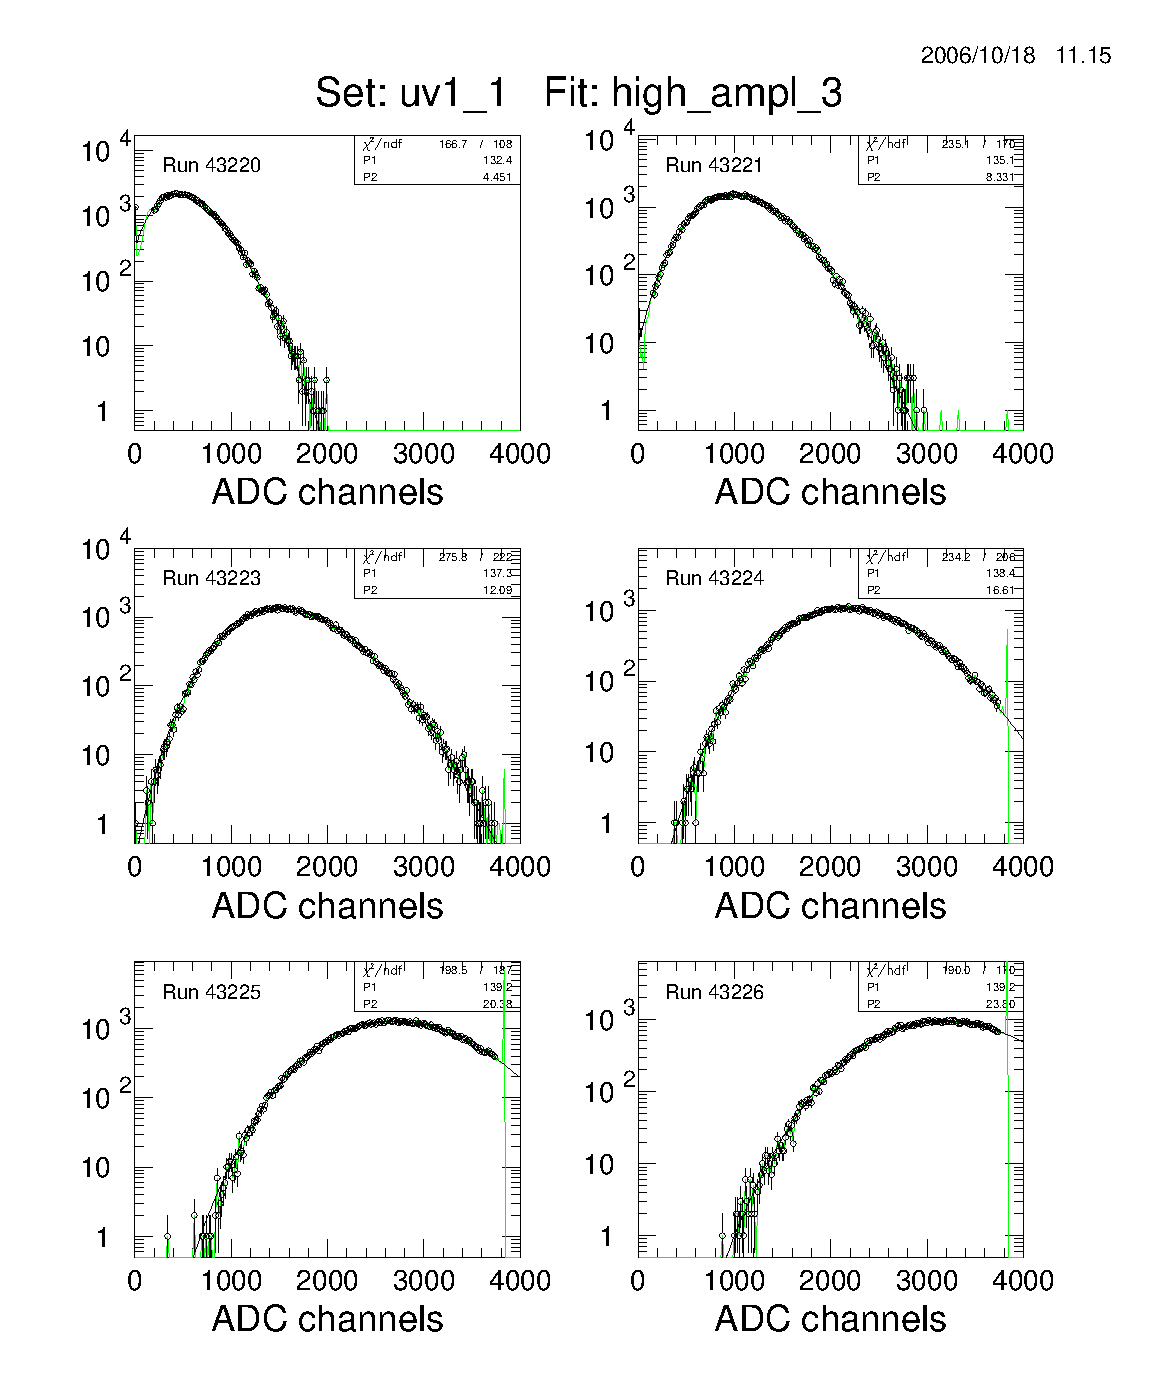
\includegraphics[height=7.5cm]{uv_1_fit.eps}
 \vspace{0.5cm}
 \caption{\label{uv_1_fit}
The LED spectra of the PMT N1. The spectra were fit by Poisson function.
P1 is the position of one-photoelectron peak. P2 is the average number of the photoelectrons.}
\end{centering}
 \end{figure}

%-------------------------------------------

 \begin{figure}
 \hspace{0.5cm}
 \begin{centering}
  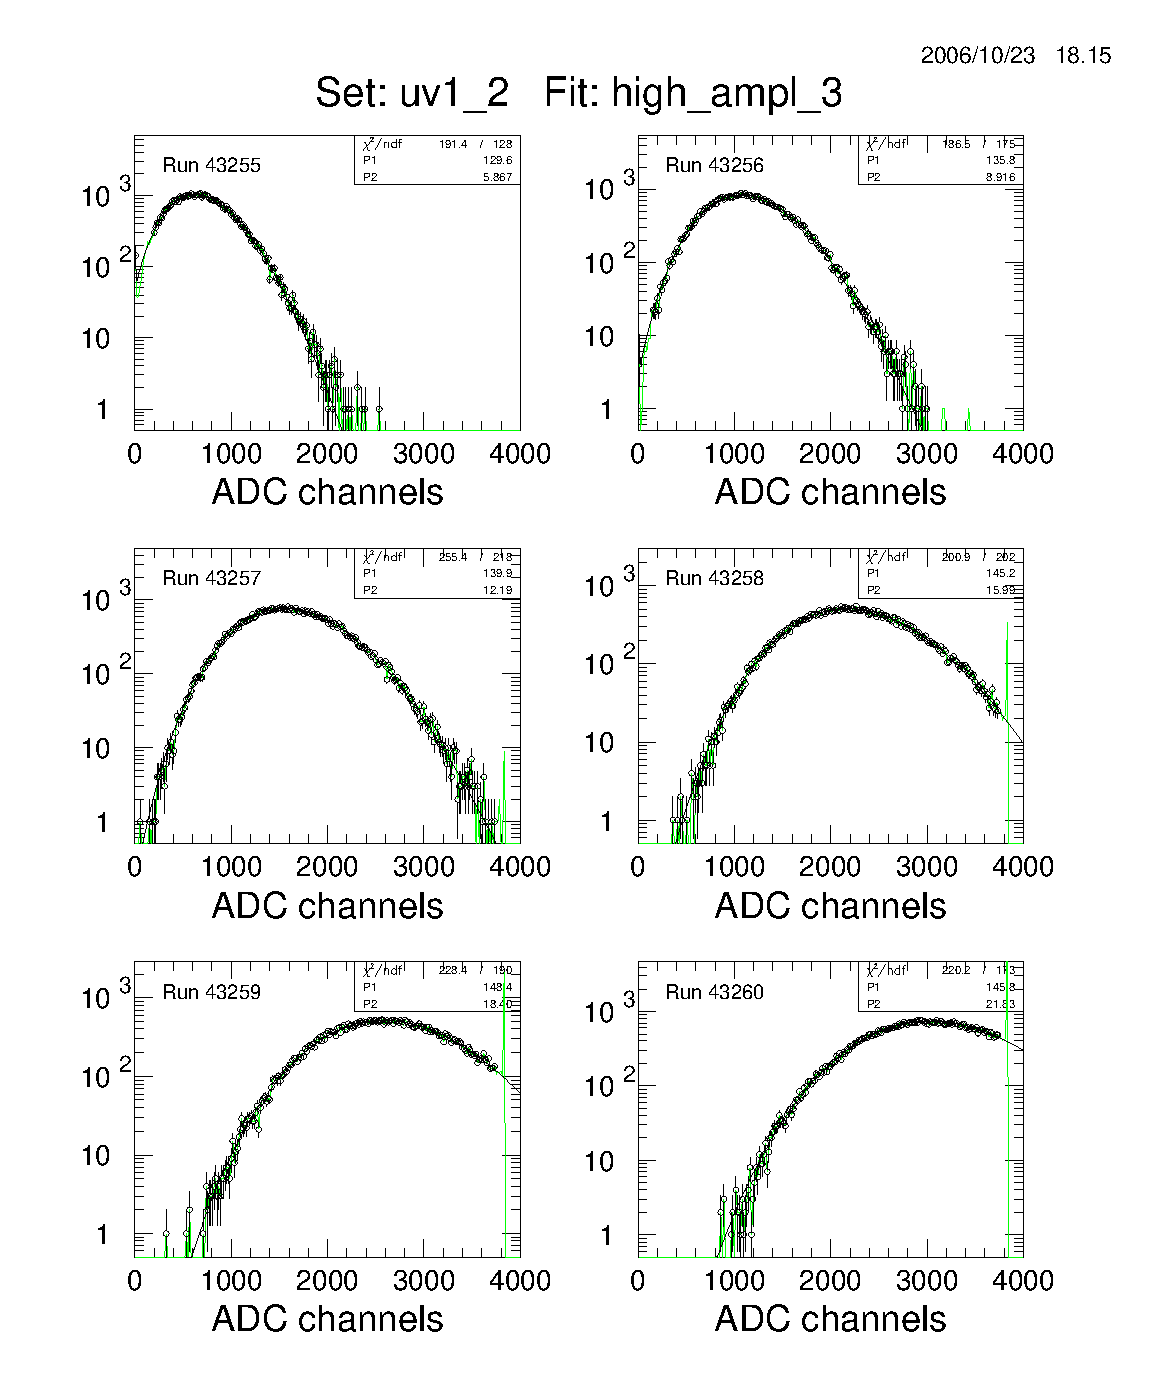
\includegraphics[height=7.5cm]{uv_2_fit.eps}
 \vspace{0.5cm}
 \caption{\label{uv_2_fit}
The LED spectra of the PMT N2. The spectra were fit by Poisson function.
P1 is the position of one-photoelectron peak. P2 is the average number of the photoelectrons.}
\end{centering}
 \end{figure}

%-------------------------------------------

 \begin{figure}
 \hspace{0.5cm}
 \begin{centering}
  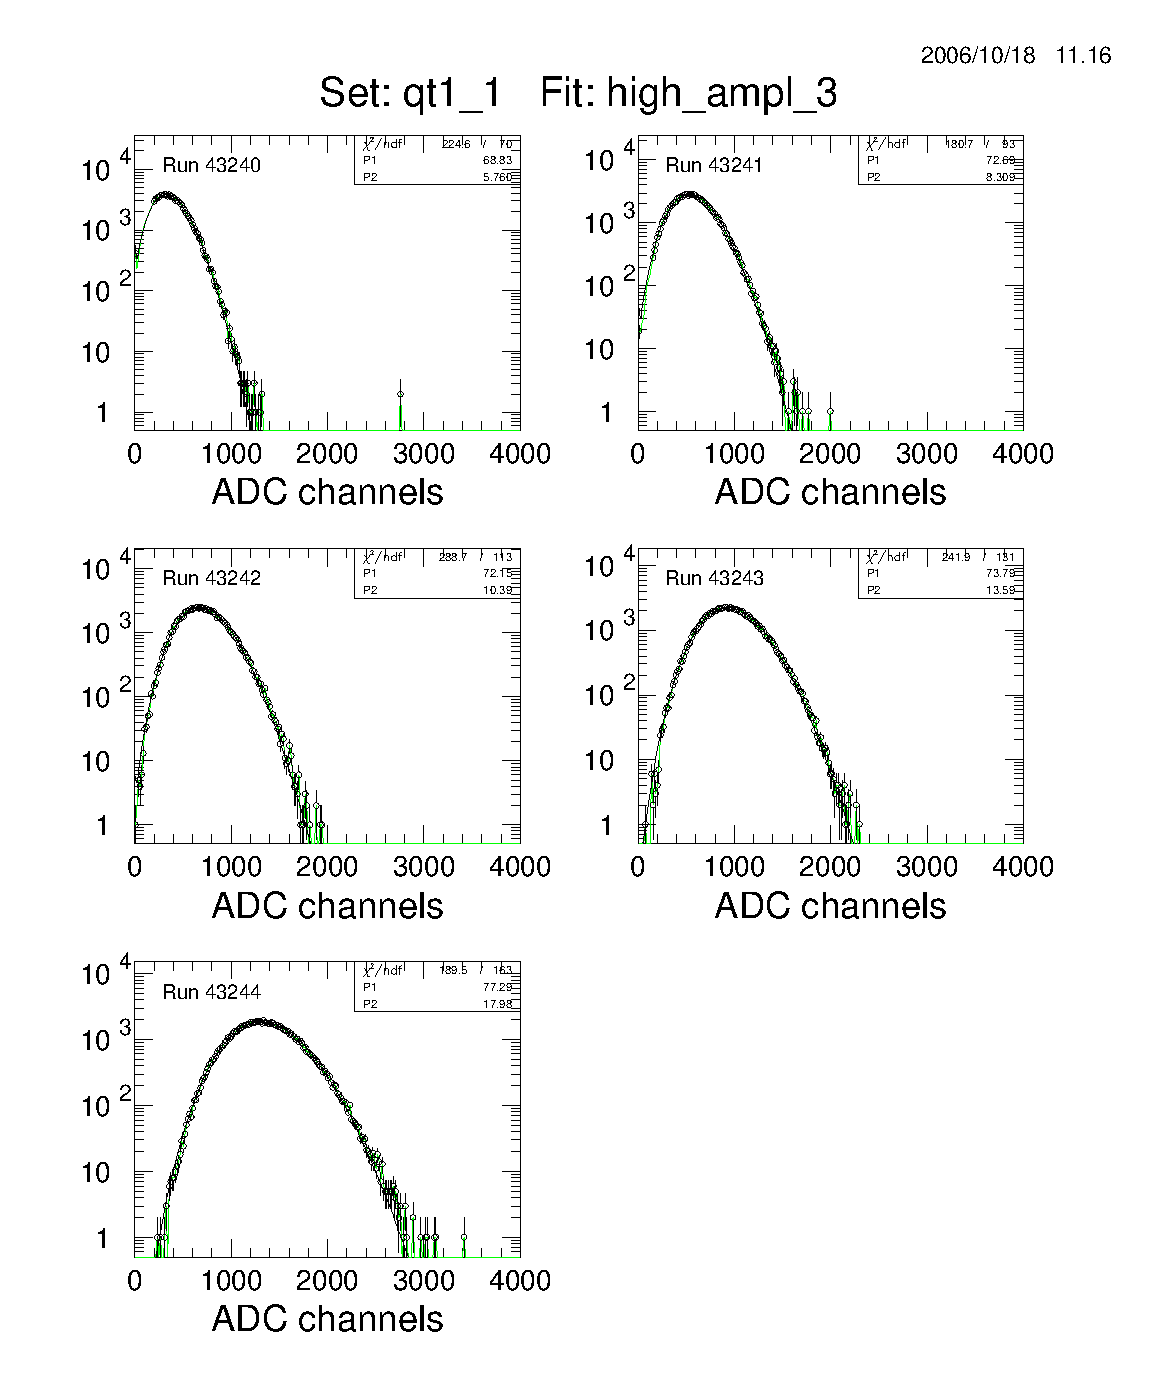
\includegraphics[height=7.5cm]{qt_1_fit.eps}
 \vspace{0.5cm}
 \caption{\label{qt_1_fit}
The LED spectra of the PMT N3. The spectra were fit by Poisson function
with two parameters; 
P1 is the position of one-photoelectron peak, P2 is the average number of the photoelectrons.}
\end{centering}
 \end{figure}

%-------------------------------------------

 \begin{figure}
 \hspace{0.5cm}
 \begin{centering}
  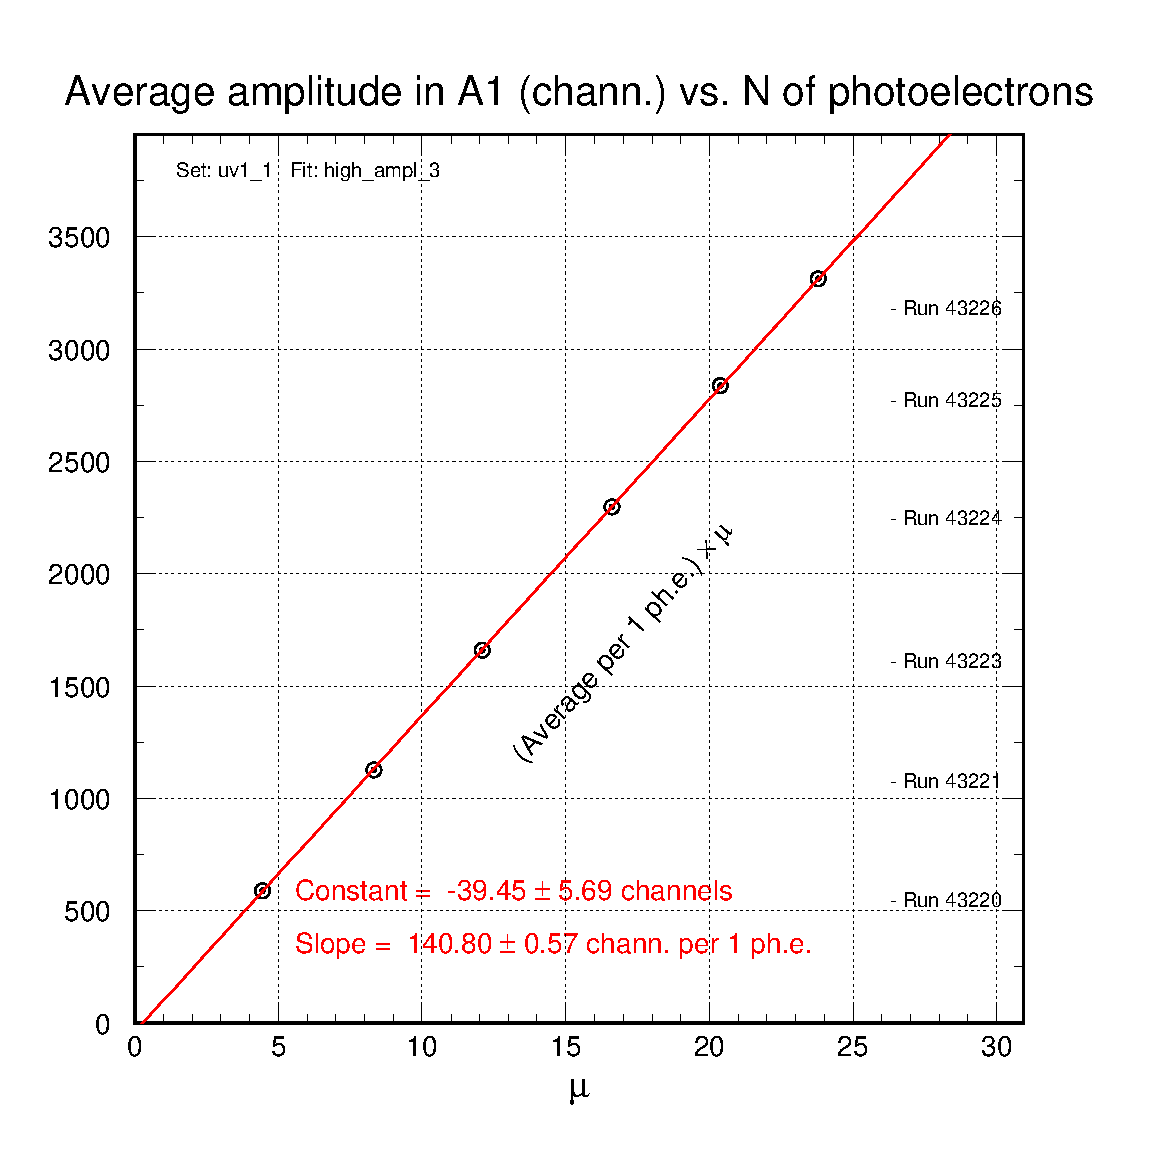
\includegraphics[height=7.5cm]{uv_1_result.eps}
 \vspace{0.5cm}
 \caption{\label{uv_1_result}
ADC value vs fitted number of the photoelectrons for PMT N1. The fit is straight line.}
\end{centering}
 \end{figure}

%-------------------------------------------

 \begin{figure}
 \hspace{0.5cm}
 \begin{centering}
  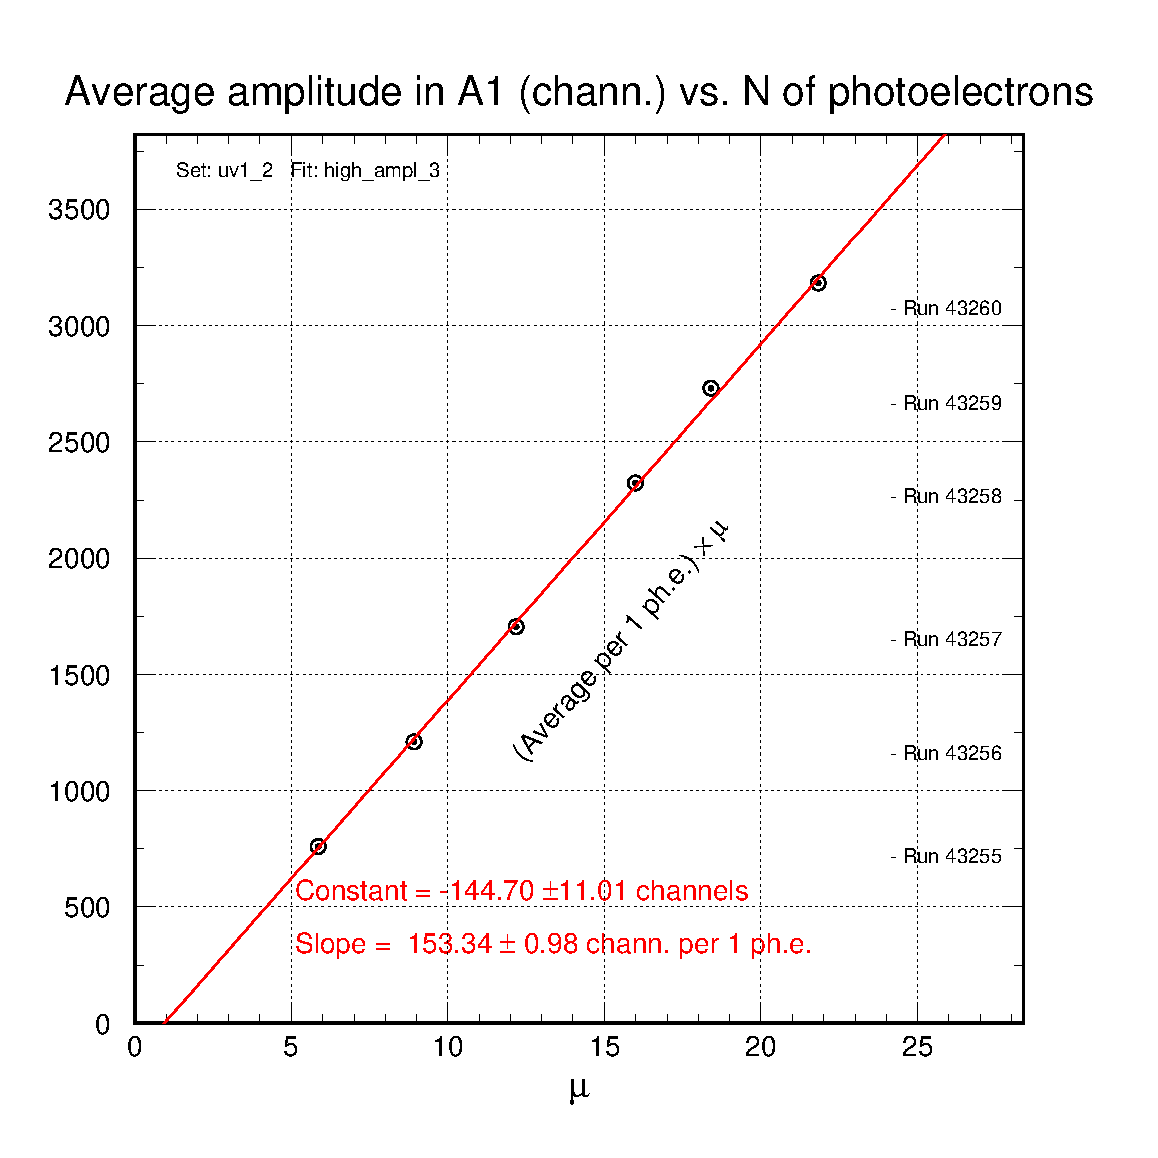
\includegraphics[height=7.5cm]{uv_2_result.eps}
 \vspace{0.5cm}
 \caption{\label{uv_2_result}
ADC value vs fitted number of the photoelectrons for PMT N2. The fit is straight line.}
\end{centering}
 \end{figure}

%-------------------------------------------

 \begin{figure}
 \hspace{0.5cm}
 \begin{centering}
  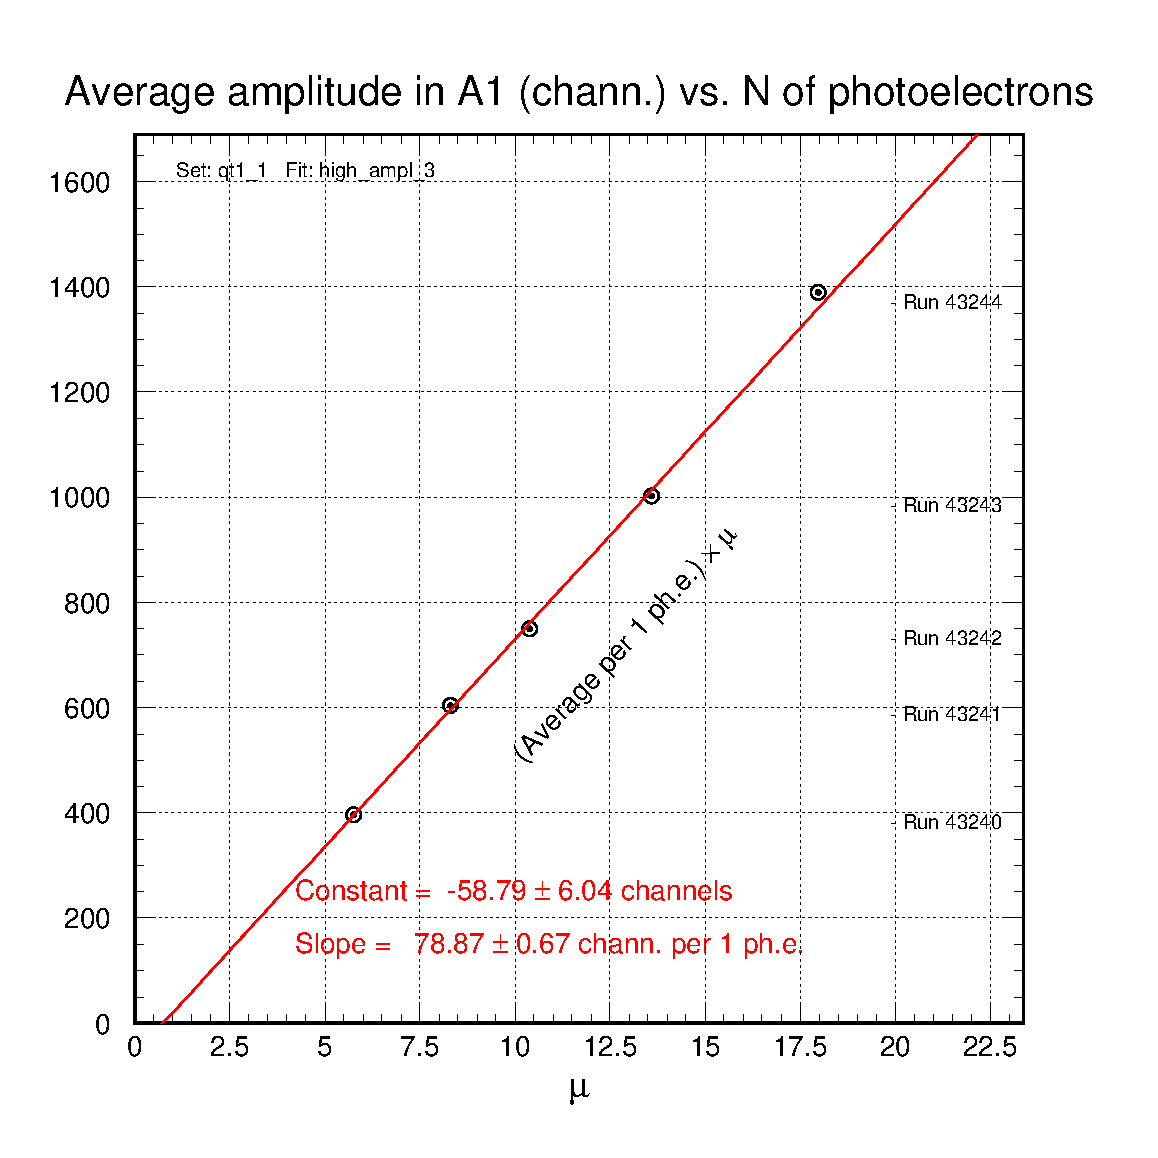
\includegraphics[height=7.5cm]{qt_1_result.eps}
 \vspace{0.5cm}
 \caption{\label{qt_1_result}
ADC value vs fitted number of the photoelectrons for PMT N3. The fit is straight line.}
\end{centering}
 \end{figure}

%------------------------------------------------ 
 \begin{figure}
 \hspace{-0.5cm}
 \begin{centering}
  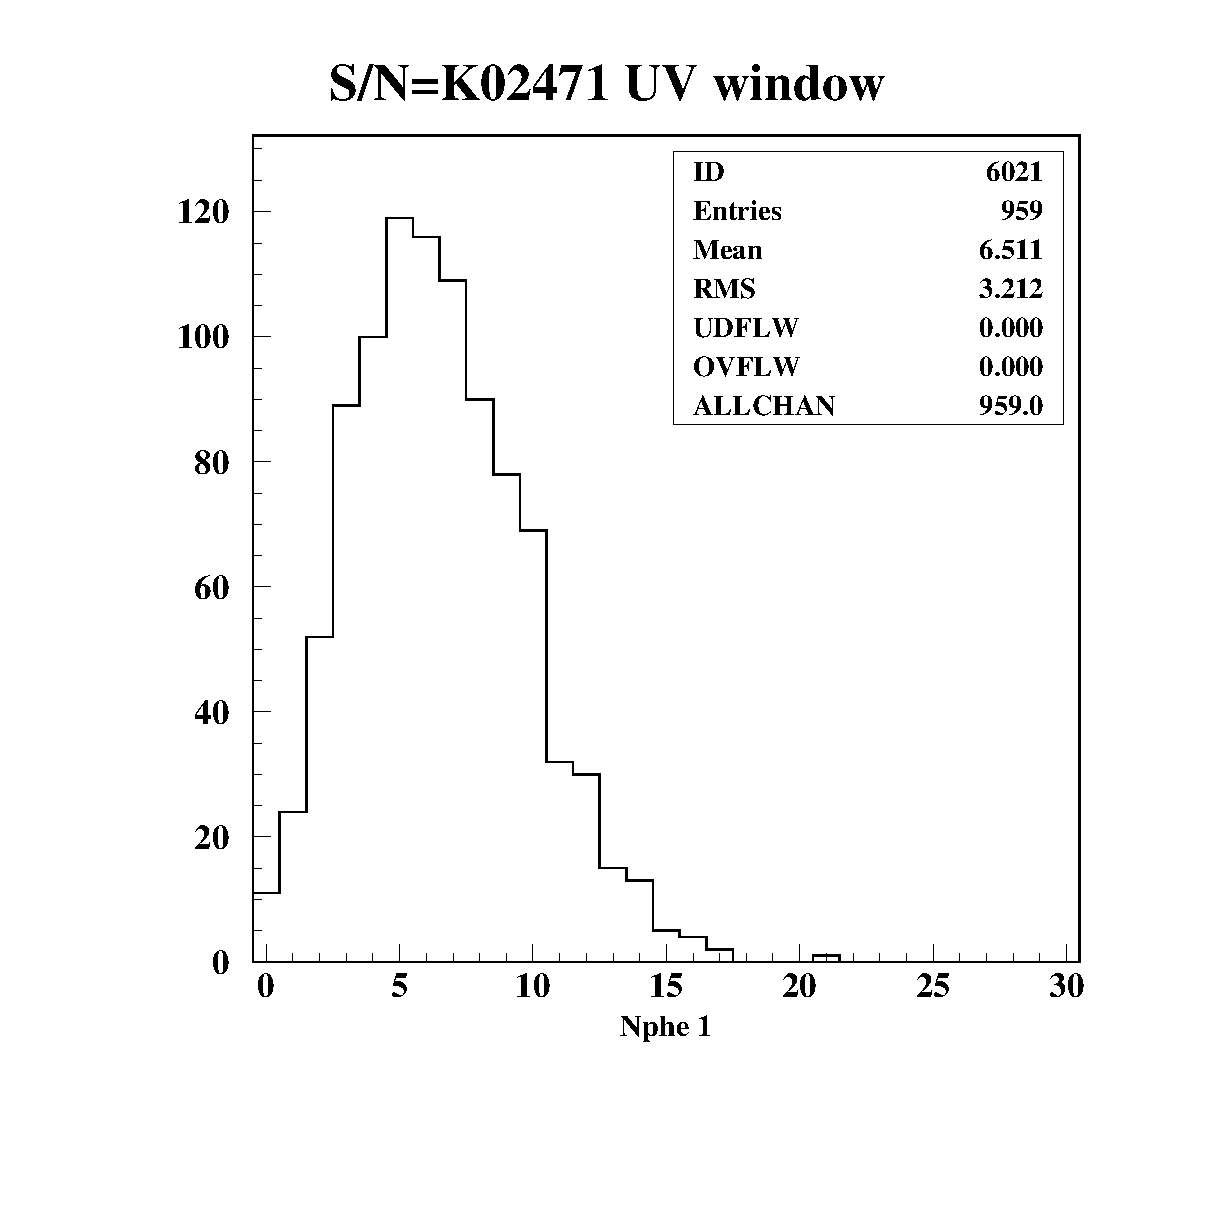
\includegraphics[height=7.5cm]{k02471_ph.eps}
 \vspace{-1cm}
 \caption{\label{stand_phe}
The distribution on the number of photoelectrons for the \v Cerenkov PMT with UV input window.}
\end{centering}
 \end{figure}

\section{Relative Quantum Efficiency Measurements}

The test stand to measure the relative quantum efficiency of different types of 
PMT's as a function of the wave length in the deep ultra-violent region is shown in 
Fig. \ref{clas12_optics}. 
The universal monochromator illuminator (Newport, model 7340).
with Deuterium lamp is used as a source of high intensity ultraviolet 
radiation down to 160 nm. It is exactly what we need for the PMTs with quartz or ultraviolet 
glass input window. The light source is directly connected with 
the Cornerstone$^{TM}$ 260 1/4 M monochromator (Newport, model 74100). It is designed
for fast, automated scanning over a broad spectral range even below 180 nm.
The signals from PMT is measured in the counting mode..


%-------------------------------------------
 \begin{figure}
 \hspace{0.5cm}
 \begin{centering}
  \includegraphics[height=5.5cm]{cerenk-stand.epsi}
 \vspace{0.5cm}
 \caption{\label{clas12_optics}
The stand for the optical test of the photomultipliers. PMT in the black cylinder
is connected by the fiber optics to the monochromator illuminator. The light source is Deuterium lamp.}
 \end{centering}
 \end{figure}

The PMT rate as a function of high voltage (HV) is shown in Fig. \ref{plateau}  
The plateau is clearly seen. The work HV is 2050 V for this particular PMT.
%-------------------------------------------
 \begin{figure}
 \hspace{0.5cm}
 \begin{centering}
  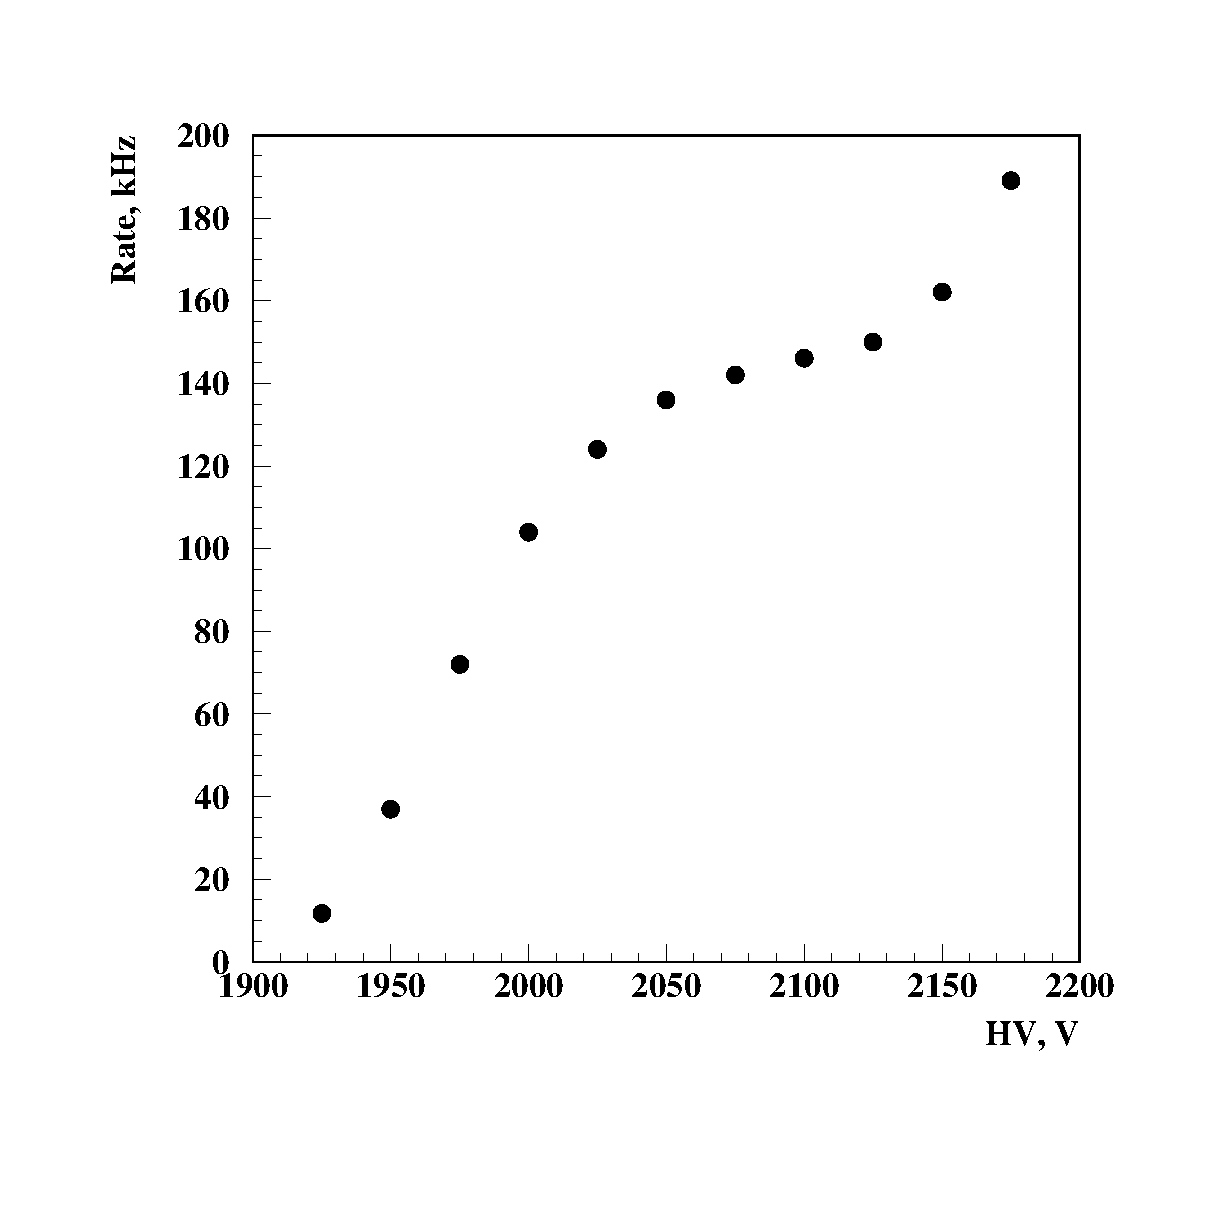
\includegraphics[height=7.5cm]{plateau.eps}
 \vspace{0.5cm}
 \caption{\label{plateau}
The PMT rate as a function of high voltage.}
 \end{centering}
 \end{figure}

Top panel of Fig.~\ref{rt_vs_wl} presents the rate as a function of the light wave length
for the PMT with quartz input window (shown in blue) and for the PMT with UV input window
(shown in red). The bottom panel shows the ratio of these rates as a function of the
wave length. It is clearly seen that PMT with quartz window started to detect photons with 
the wave length greater than 180 nm. At the same time the PMT with UV input window has 
the threshold near 220--240 nm. This is extremely important for the detection of  \v Cerenkov
light. The   \v Cerenkov light spectrum behaves as $dN/d\lambda \sim 1/\lambda^2$.
The ratio  $R={N_{phe}^{Quartz} \over N_{phe}^{UV}}=0.5$ at $ \lambda=230$ nm.
We can estimate the ratio of the detected photoelecrons for these two type of PMT as

$ R={N_{phe}^{Quartz} \over N_{phe}^{UV}}={\lambda_{threshold}^{quartz} \over \lambda_{threshold}^{UV}}\sim {230\over 180}\sim 1.3 $

This is expected increase of the detected number of photoelecrons for the qurtz PMT in comparison with
the UV PMT.

%-------------------------------------------
 \begin{figure}
 \hspace{0.5cm}
 \begin{centering}
  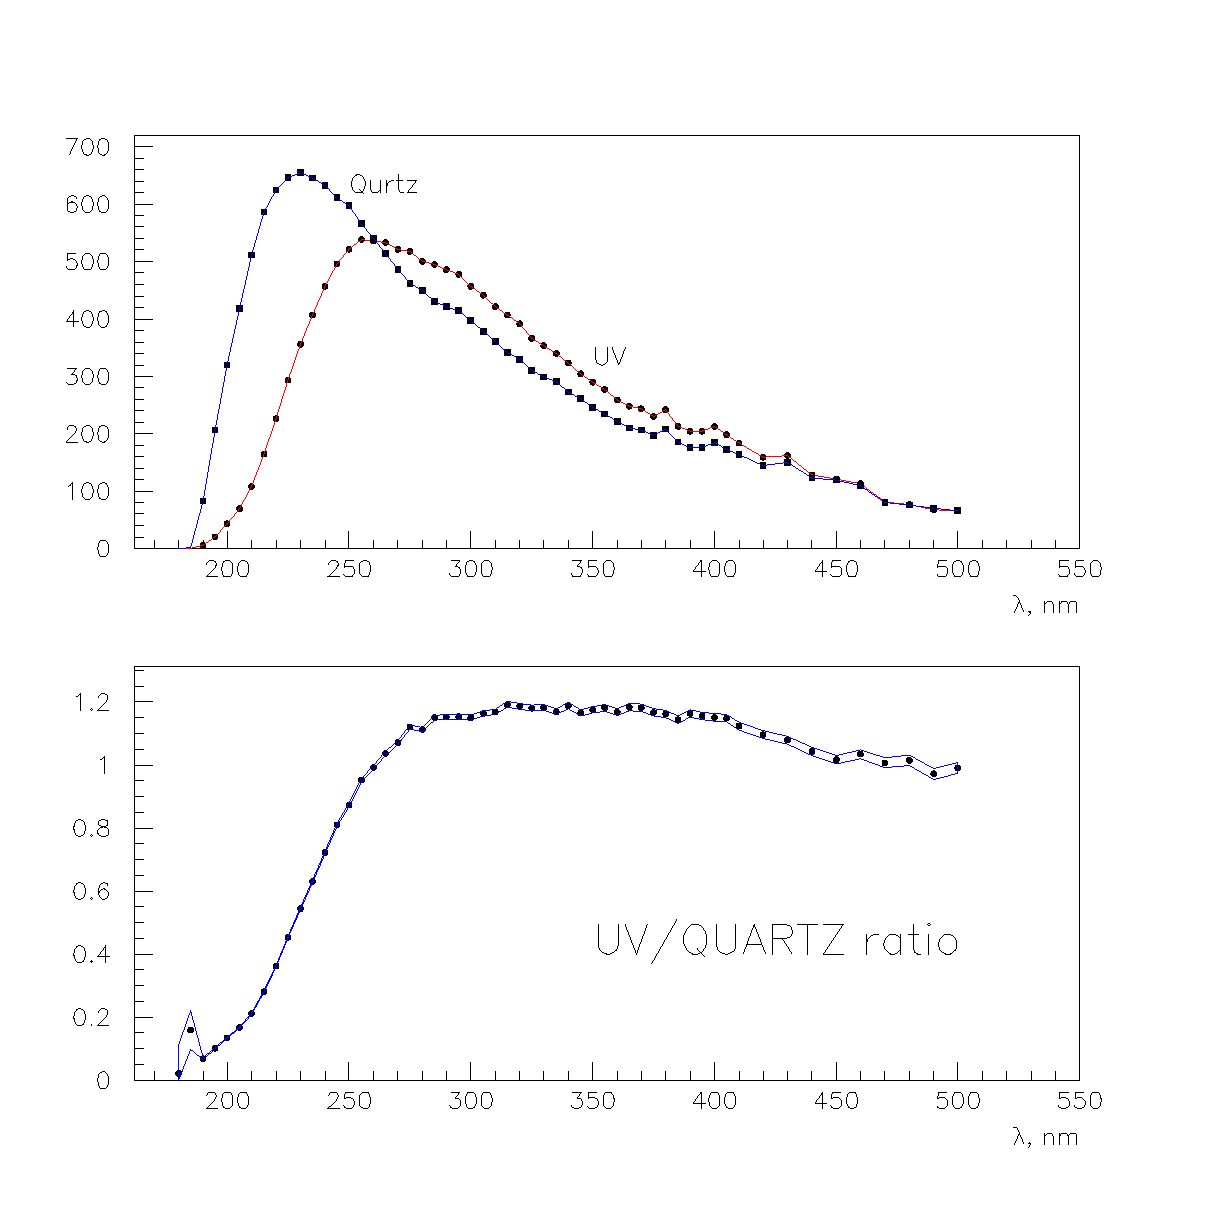
\includegraphics[height=7.5cm]{rate_vs_wl.eps}
 \vspace{0.5cm}
 \caption{\label{rt_vs_wl}
Top panel: the PMT rate as a function of the light wave length
for the PMT with quartz window (in blue) and with UV-window (in red).
Bottom panel: the ratio of these rates}
 \end{centering}
 \end{figure}

\section{PMT magnetic shielding}
%-------------------------------------------
 \begin{figure}
 \hspace{0.5cm}
 \begin{centering}
  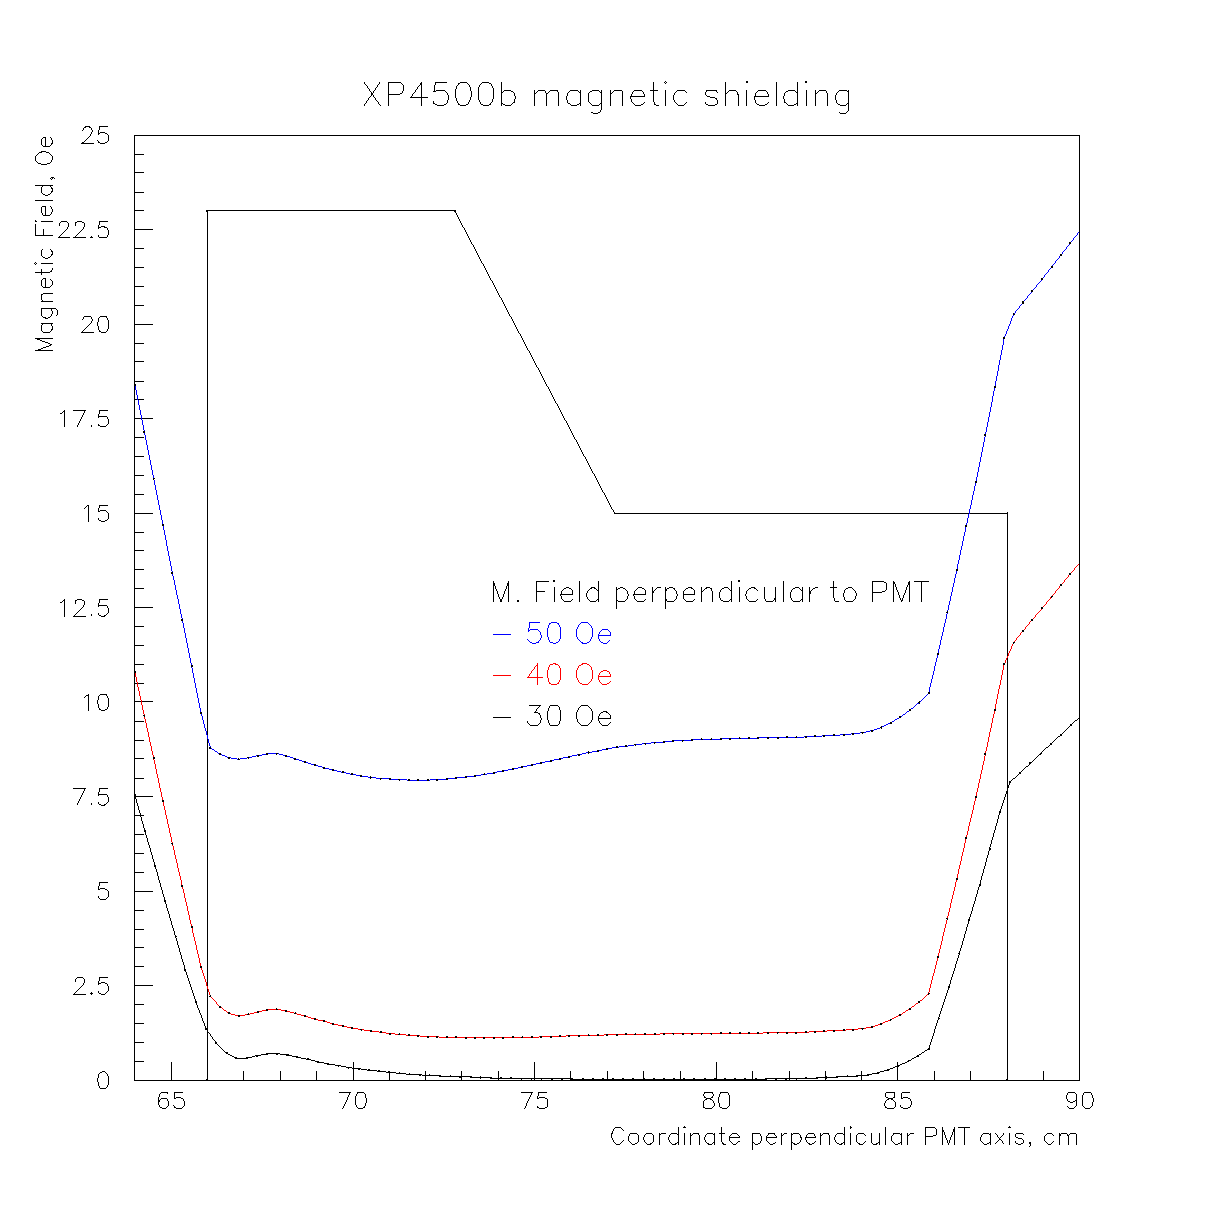
\includegraphics[height=7.5cm]{shield_r_lin.eps}
 \vspace{0.5cm}
 \caption{\label{lin_r}
Standard single layer PMT magnetic shielding (shown in black).
Magnetic field perpendicular to the PMT axis.
50 gauss field is shown in blue, 40 gauss - in red, 30 gauss in black.
}
\end{centering}
 \end{figure}
%-------------------------------------------
 \begin{figure}
 \hspace{0.5cm}
 \begin{centering}
  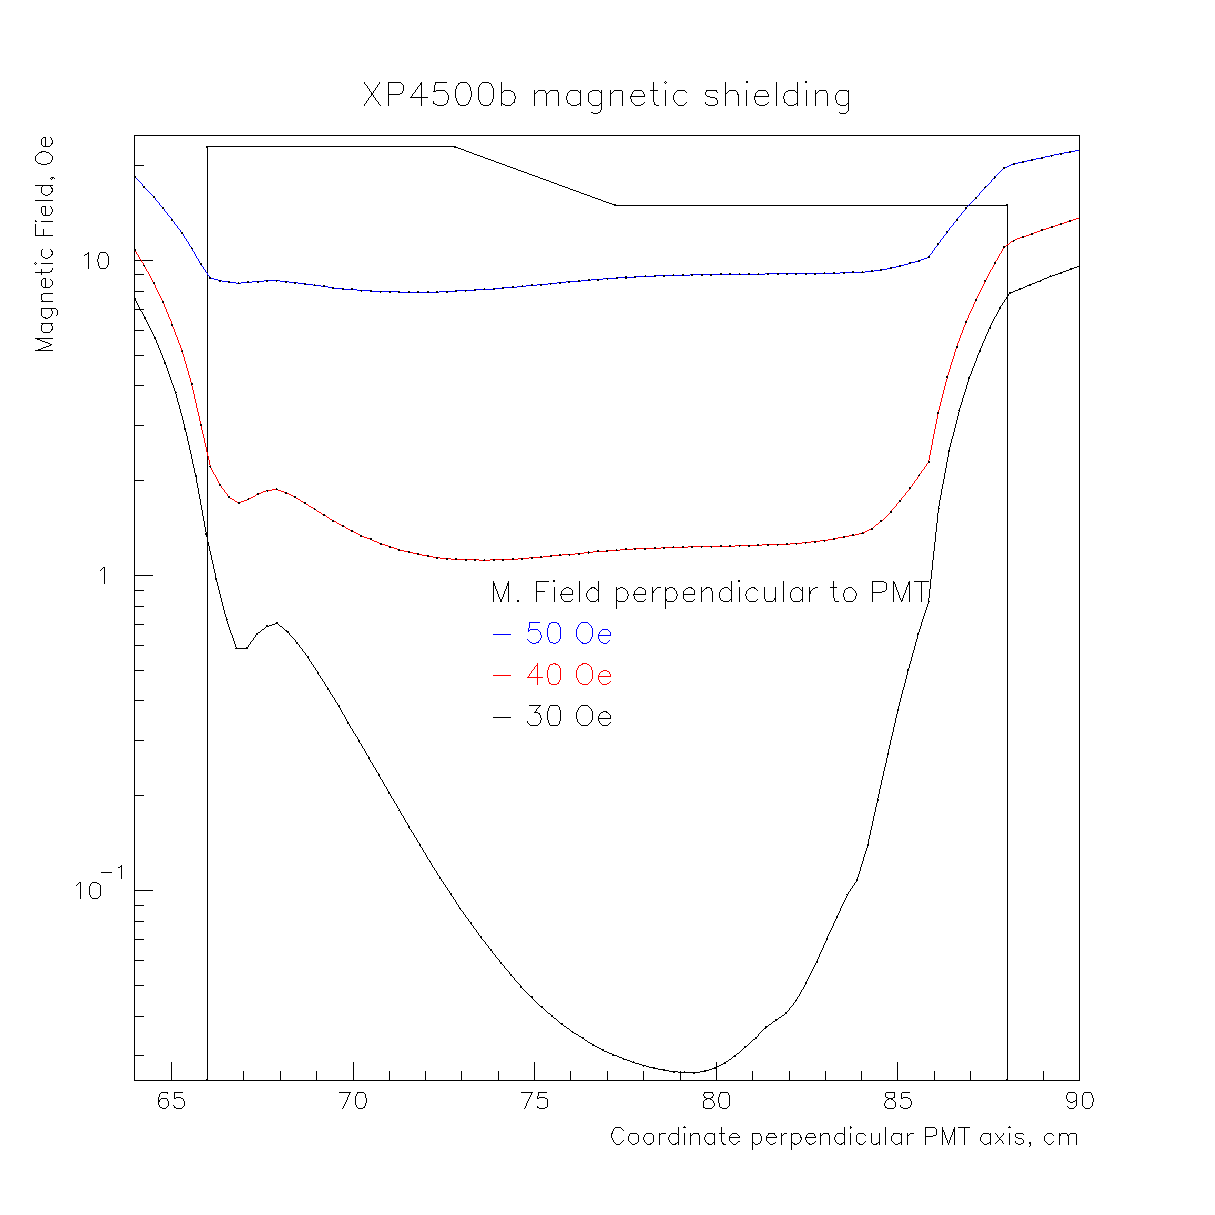
\includegraphics[height=7.5cm]{shield_r_log.eps}
 \vspace{0.5cm}
 \caption{\label{log_r}
Same as Fig.~\ref{lin_r} but with logarithmic y axis.}
\end{centering}
 \end{figure}
%-------------------------------------------
 \begin{figure}
 \hspace{0.5cm}
 \begin{centering}
  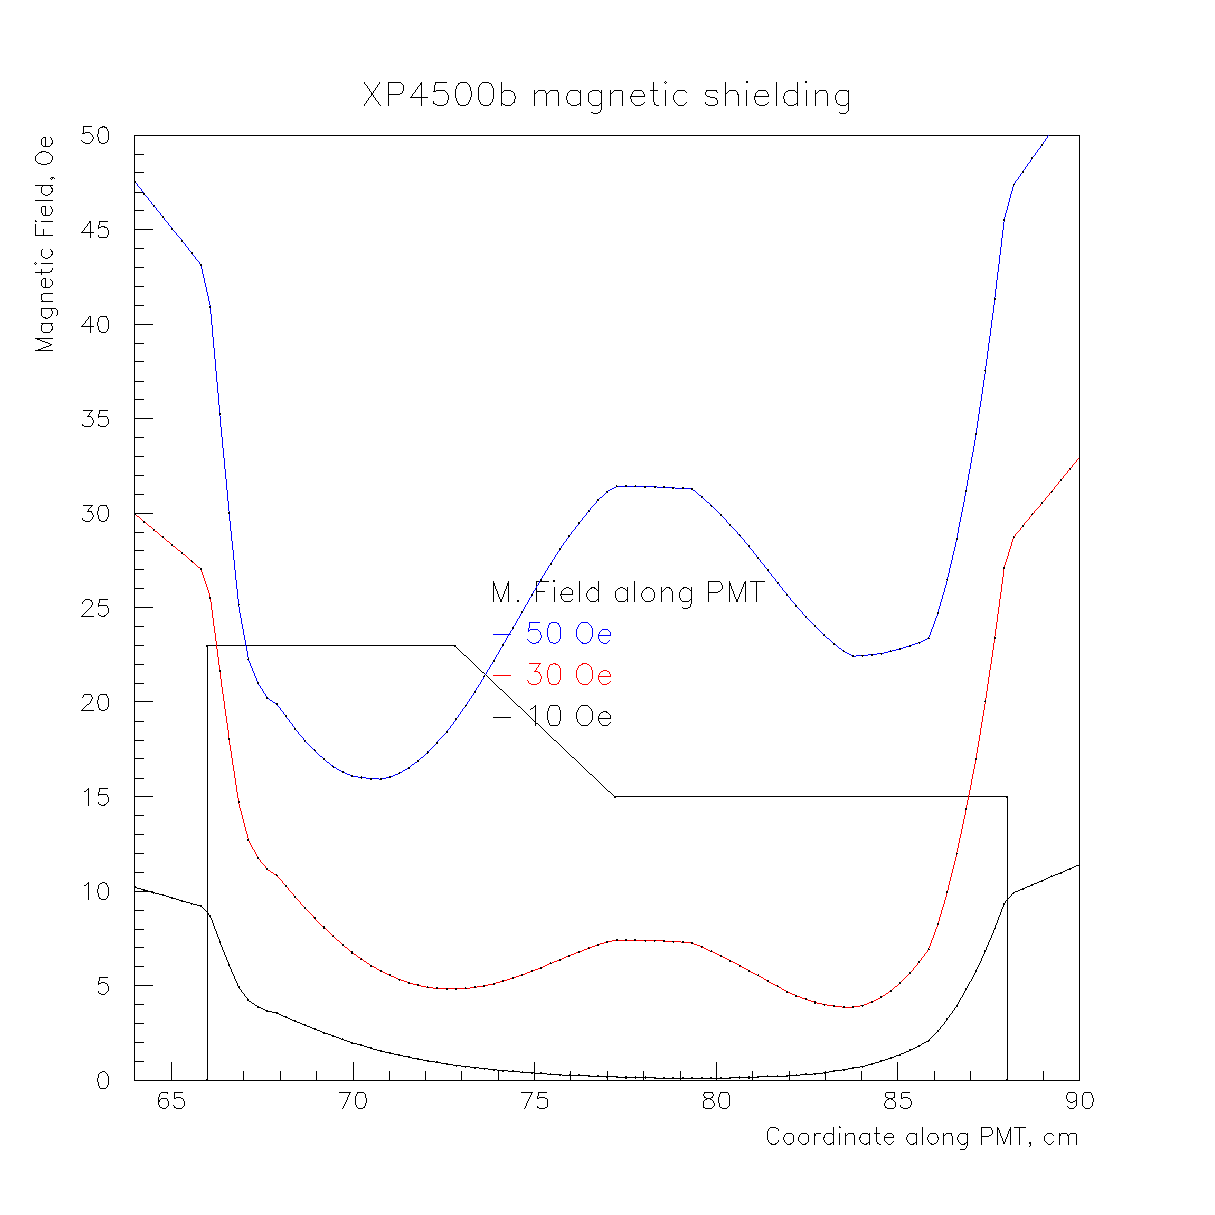
\includegraphics[height=7.5cm]{shield_z_lin.eps}
 \vspace{0.5cm}
 \caption{\label{lin_z}
Standard single layer PMT magnetic shielding (shown in black).
Magnetic field along the PMT axis.
50 gauss field is shown in blue, 40 gauss - in red, 30 gauss in black.
}
\end{centering}
 \end{figure}
%-------------------------------------------
 \begin{figure}
 \hspace{0.5cm}
 \begin{centering}
  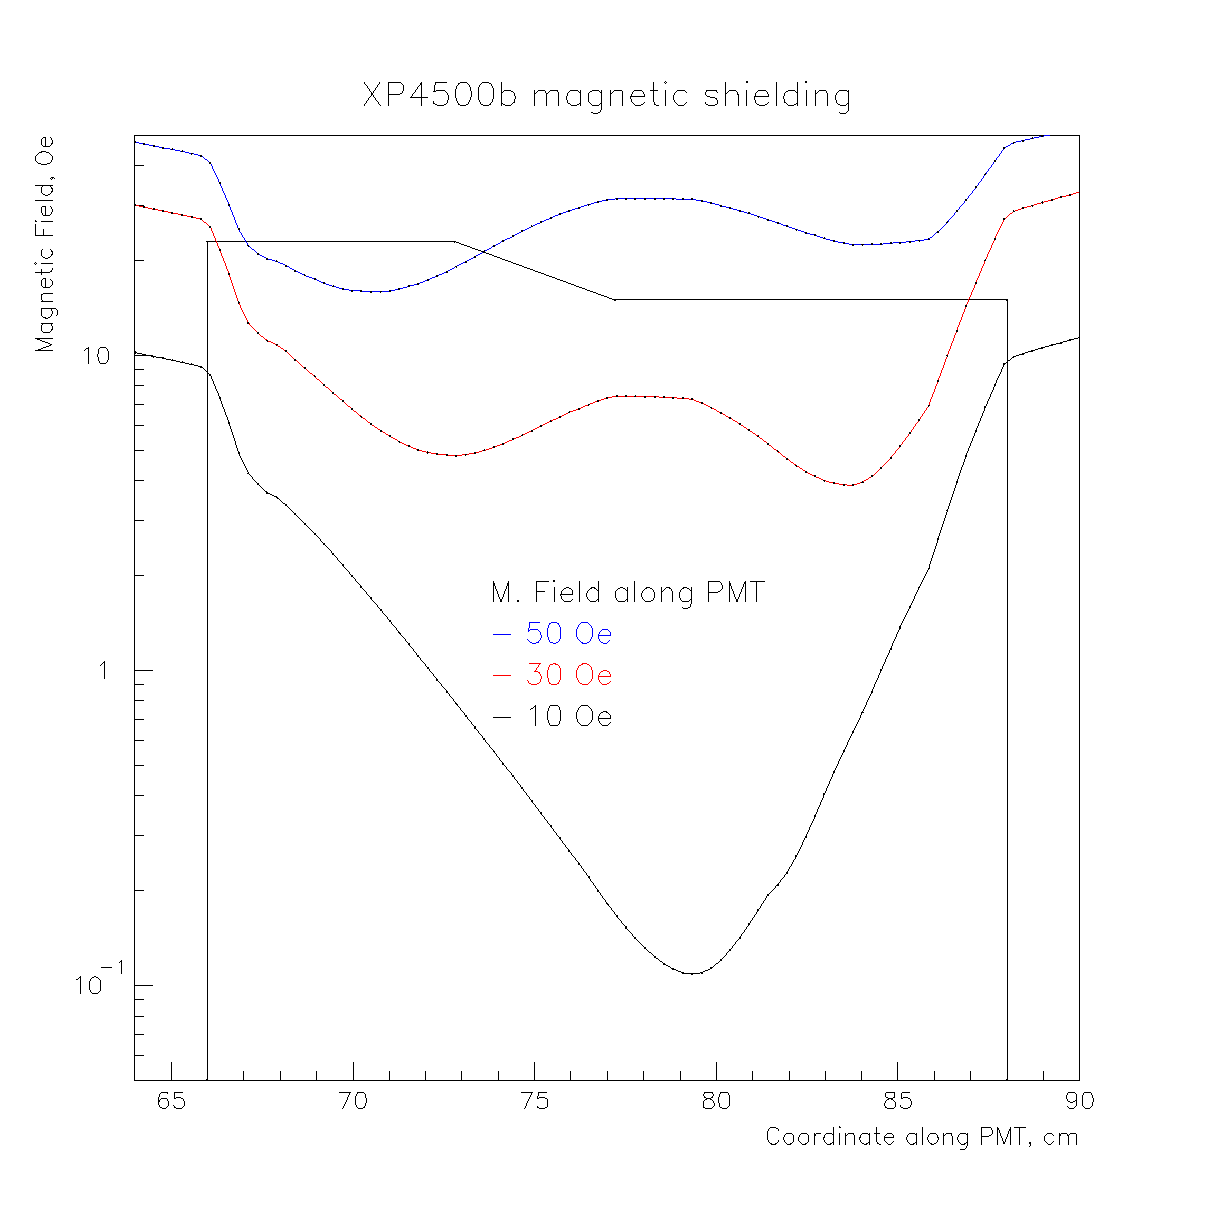
\includegraphics[height=7.5cm]{shield_z_log.eps}
 \vspace{0.5cm}
 \caption{\label{log_z}
Same as Fig.~\ref{lin_z} but with logarithmic y axis.}
\end{centering}
 \end{figure}

The PMT of the \v Cerenkov counter will be located in the region with the magnetic field.
The maximum magnetic field was estimated for the current design as 50 gauss.
The PMT gain halved for a magnetic field
\begin{itemize}
\item perpendicular to the PMT axis      - 0.4 gauss
\item parallel with the PMT axis - 1.3 gauss
\end{itemize}
The standard PMT magnetic shield is not enough to have residual field at the level of 0.4-1 gauss
for 50 gauss magnetic field..
We made the calculation of the residual magnetic field using TOSKA program.
Fig.\ref{lin_r},\ref{log_r},\ref{lin_z},\ref{log_r} present the residual magnetic field at the PMT axis
for standard single layer PMT magnetic shielding for three values of the  magnetic field:
50, 40, and 30 gauss with the direction of the magnetic field perpendicular and parallel the PMT axis
(linear and logarithmic y scales are shown).
In the first case the residual magnetic field inside the PMT volume is around 8, 2, and 1 
gauss for the magnetic  field 50, 40, and 30 gauss respectively. 
For the second case (the field is along the PMT axis) the residual is sufficiently higher.
The residual magnetic field inside the PMT volume is around 30, 10, and 1-2  
gauss for the magnetic  field 50, 40, and 30 gauss respectively.
We may conclude from this calculation that
\begin{itemize}
\item We need additional magnetic shielding to suppress the residual magnetic field 
      to the level of 0.5 gauss.
\item The residual  field is significantly (several times) higher when the magnetic field is directed along the PMT axis.
\item The shielding needs to extend beyond the PMT window for at least one diameter.
\end{itemize}

We model three layers magnetic field shielding configuration using TOSKA program.
Fig.~\ref{3layers} presents the residual field for 3 different configurations
with cylindrical 1 mm thickness PMT magnetic shielding  with the magnetic directed along the PMT axis.
\begin{itemize}
\item Single layer tube made of  co-netic $\mu$ metal (shown in black)
\item Two layers  made of  Tc and co-netic $\mu$ metals (shown in red)
\item Three layers  made of  netic, co-netic, and co-netic $\mu$ metals (shown in blue)
\end{itemize}

The residual magnetic field with three layer shielding is below 1 gauss in the region
$\pm$ 5 cm. It is inside the specs for the parallel to the PMT axis magnetic field.
The perpendicular field will be several times lower as we can conclude from our calculations with
standard PMT magnetic shielding.


%-------------------------------------------
 \begin{figure}
 \hspace{0.5cm}
 \begin{centering}
  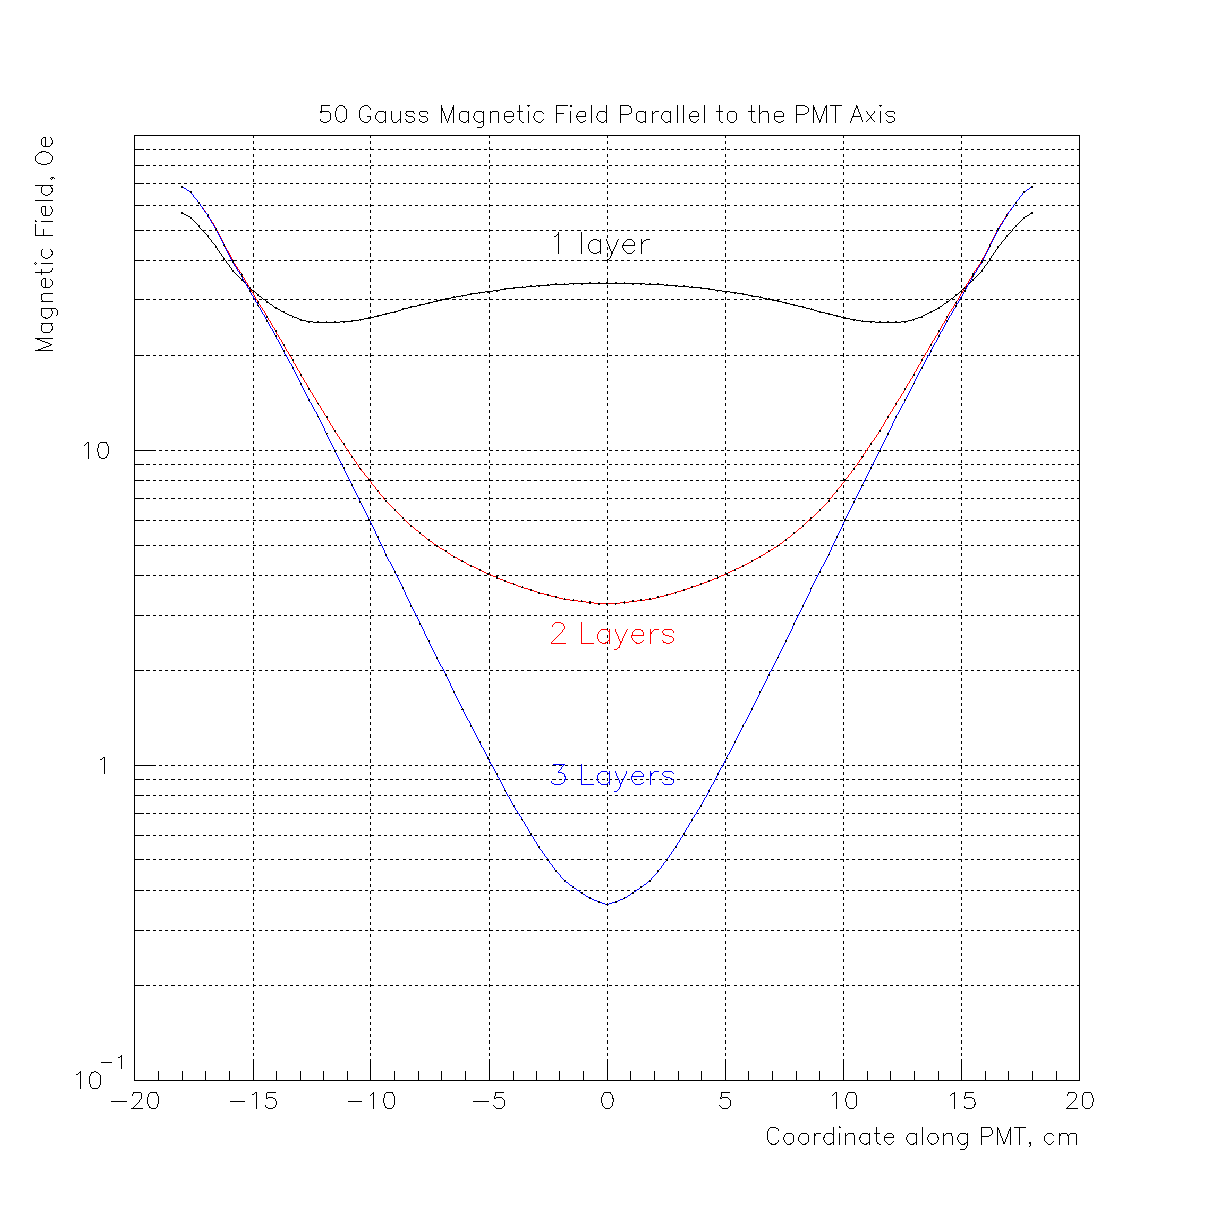
\includegraphics[height=7.5cm]{3layers.eps}
 \vspace{0.5cm}
 \caption{\label{3layers}
The cylindrical PMT magnetic shielding.
Magnetic field along  the PMT axis (50 gauss).
Single layer shielding is shown in black.
Two layers shielding is shown in red.
Three layers shielding is shown in blue.}
\end{centering}
 \end{figure}



\end{document}





